\chapter{Ръководство на потребителя}
	За използване на системата е необходима библиотеката \emph{Moai SDK},
	версия в диапазона 1.0-1.2 и \emph{Windows} базирана система. Стартирането
	става чрез файла ''run.bat''. При изпълнението на файла на екрана на потребителя
	се изобразява нещо подобно на \ref{fig:simulation-screen}. Изобразява се
	екран с модели, готови за работа и работеща симулация. Горе в дясно, потребителят,
	може да наблюдава изминалото време от симулацията.
	
	След удовлетворяване на условието за край на симулацията, на екранът се изобразява
	статистика, представляваща различни метрики от симулацията. Подобна такава е представена
	на \ref{fig:result-screen}. Представената информация е:
	
	\begin{itemize}
		\item \emph{Running Time} време, за което симулацията се е изпълнявала
		\item \emph{Vehicles Passed} броят модели, които са успели да преминат кръстовището
		\item \emph{Congestion Factor} метрика, показваща ефективността на използваната стратегия. 
			По-голяма стойност - по-добър резултат.
	\end{itemize}
	
	Използваната стратегия за симулация по подразбиране е \emph{simple}, която дава
	време от 3 секунди зелена светлина на всяка страна от кръстовището. Друг предоставен
	алгоритъм е \emph{bus-priority}. Тази стратегия дава зелена светлина на първия срещнат автобус,
	независимо от текущото състояние на кръстовището.
	
	\begin{figure}[htb]
		\centering
		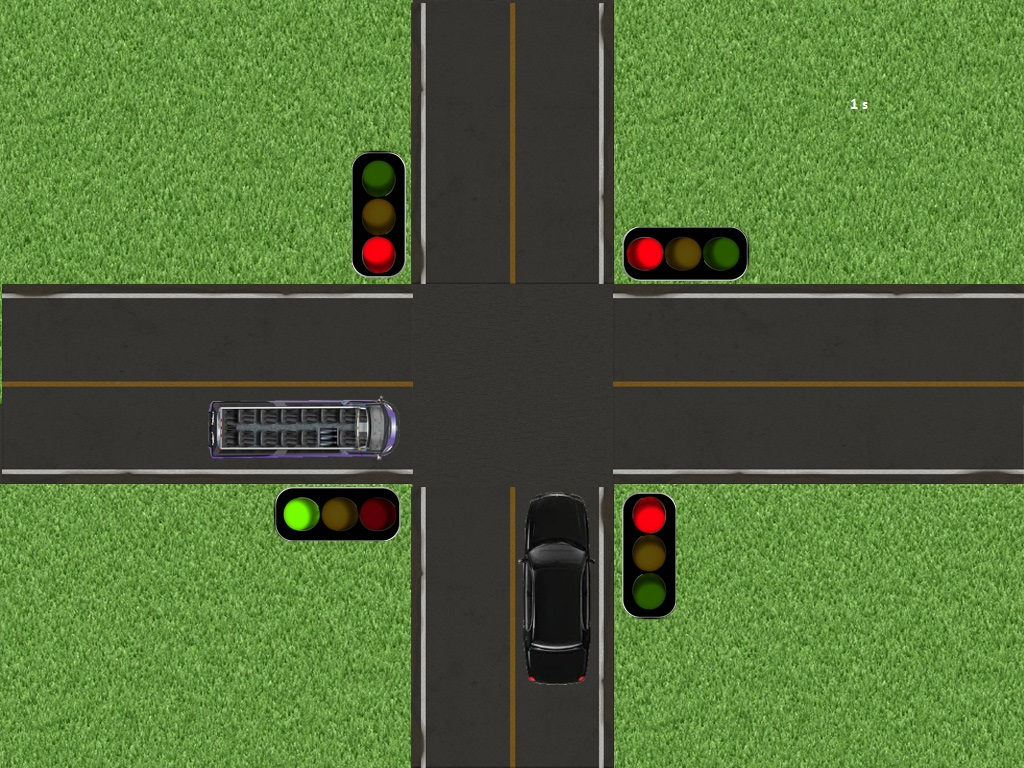
\includegraphics[scale=0.4]{assets/simulation.jpg}
		\caption{Екран при стартиране}
		\label{fig:simulation-screen}
	\end{figure}
	
	\begin{figure}[htb]
		\centering
		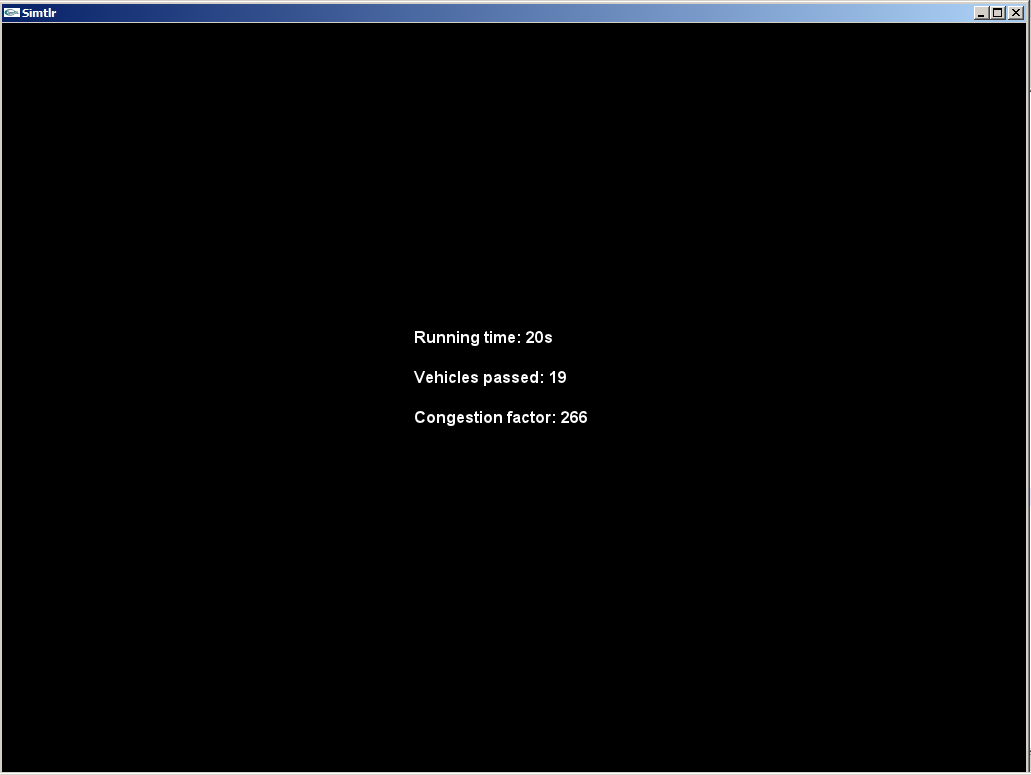
\includegraphics[scale=0.4]{assets/result.png}
		\caption{Екран след приключване на симулация}
		\label{fig:result-screen}
	\end{figure}	
	
	\subsubsection{Конфигурация}
	
		За конфигуриране на симулационната система се използва файла \emph{config.lua}, намиращ се в директорията \emph{src}.
		В нея може да се променят следните симулационни настройки:
		
		\begin{itemize}
			\item \emph{STRATEGY} - избор на използваната стратегия за симулацията
			\item \emph{TOTAL RUNNING TIME} - времето за което симулацията е активна
			\item \emph{MAXIMUM MODELS PER SIDE} - максималния брой модели, които могат да бъдат поставени в опашката на някоя
			от страните на кръстовището
		\end{itemize}
		
		За конфигурарине на коефициентите на ефективност в кръстовището се използват:
		
		\begin{itemize}
			\item \emph{BUS EFFECTIVENESS MULTIPLIER} - определя коефициент на ефективност за автобуси
			\item \emph{CAR EFFECTIVENESS MULTIPLIER} - определя коефициент на ефективност за коли
		\end{itemize}
		